\documentclass{article}

\usepackage{enumerate}
\usepackage{makecell} 
\usepackage{graphicx}
\usepackage{pgfgantt}
\usepackage[section]{placeins}
\usepackage[spanish]{babel}
\usepackage[utf8]{inputenc}

\begin{document}
  \title{%
  Protocolo \\
  \large Revisión de la literatura sobre las actividades de requisitos para Software como Servicio\\}
  \author{Alberto de Jesús Sánchez López \\ 
  \small Proyecto Guiado}
  \date{Fecha}
  \maketitle
  \thispagestyle{empty}
  \newpage

  \tableofcontents
  \thispagestyle{empty}
  \newpage

\setcounter{page}{1}
\section{Introducción}
Llevar a cabo un proceso de desarrollo de software que resulte en un producto de calidad, es 
un proceso complejo, que utiliza metodologías y estrategias adecuadas para el análisis del problema 
en cuestión asì cómo el diseño de una solución, para el Software como Servicio (SaaS), esta no es la excepción. 
El Software como Servicio tiene necesidades específicas que evitan la adaptación de metodologías y estrategias 
tradicionales utilizadas dentro de la Ingeniería de Software, esto representa un conjunto de problemas para aquellos 
interesados en iniciar el desarrollo de un software como servicio.

El proceso de desarrollo de software tradicional conlleva un conjunto de fases con el propósito común de asegurar la entrega 
de un producto con calidad y en tiempo, la fase de requisitos, es crucial para delimitar el alcance del proyecto, analizar, 
documentar y verificar los servicios y restricciones del sistema. Una definición de requisitos que ha sido desarrollada siguiendo una 
metodogìa o estrategia, es de suma importancia para el éxito del proyecto, ya que esto asegura que la especificación de requisitos ha sido 
desarrollada siguiendo un proceso formal y por ende los fundamentos necesarios para el correcto diseño de la solución son confiables.

Es por eso, que es de especial interés para aquellos involucrados en el desarrollo de un proceso que resulte en un producto de software 
con calidad. Una fase crucial para el éxito de un proyecto de software es la definición de requisitos. 
\newpage

\section{Preguntas de investigación}
El objetivo de la Revisión Sistemática de la Literatura es encontrar el estado del arte del las actividades de requisitos para un \emph{software} como servicio. 

\begin{enumerate}[P 1.-]
  \item\emph{¿Qué técnicas de elicitación se han utilizado para la identificación de requisitos de Software como Servicio?}
  \begin{enumerate}[(a)]
  \item \emph{¿Qué técnicas de elicitación se aplican?}
  \item \emph{¿Qué retos se presentan en la elicitación?}
  \end{enumerate}
  Motivación: Señalar el conjunto de técnicas utilizadas para llevar a cabo un proceso de elicitación de requisitos para un software como servicio e identificar los retos encontrados en el proceso de elicitación. 
  
  \item\emph{¿Qué técnicas de análisis se han utilizado para la definición de requisitos de Software como Servicio?}\\
  Motivación: Identificar las actividades realizadas para llevar a cabo el proceso de análisis, clasificación y definición de un conjunto de requisitos para un software como servicio.

  \item\emph{¿Qué actividades se han utilizado para llevar a cabo la validación de los requisitos de un Software como servicio?}\\
  Motivación: Identificar las técnicas que utilizadas para definir un proceso de validación de requisitos para un software como servicio.

  \item\emph{¿Qué actividades se han utilizado para gestionar los cambios de requisitos de un Software como Servicio?}
  \begin{enumerate}[(a)]
  \item \emph{¿Cómo se evalúan los cambios en los requisitos?}\
  \end{enumerate}
  Motivación: Señalar las actividades utilizadas para gestionar cambios de requisitos en un software como servicio encontradas en la literatura.
            
  \item\emph{¿Qué actividades se han utilizado para gestionar riesgos asociados a los requisitos de un Software como Servicio?}
  \begin{enumerate}[(a)]
  \item \emph{¿Cómo se identifican los riesgos?}
  \item \emph{¿Cómo se controlan los riesgos?}
  \end{enumerate}
  Motivación: Identificar las actividades utilizadas para señalar y controlar los riesgos relacionados a cambios de requisitos en un software como servicio. 
  
  \item\emph{¿Qué temas abiertos se identifican en la literatura reciente en el desarrollo de software como servicio?}
  \begin{enumerate}[(a)]
  \item \emph{¿Qué temas abiertos existen relacionados a las actividades llevadas a cabo en la gestión de requisitos de un software como servicio?}
  \end{enumerate}
  Motivación: Identificar los temas abiertos sugeridos en la literatura relacionada a las actividades de elicitación, análisis, validación y gestión de cambios 
 para requisitos de un software como servicio.
\end{enumerate}


\section{Estrategia de búsqueda}




\subsection{Términos de búsqueda}
Los siguientes términos de búsqueda fueron seleccionados con el propósito de identificar los estudios que 
permiten proveer evidencia relevante a las preguntas de investigación definidas posteriormente. 
Para lograr lo antes mencionado, se llevaron a cabo un conjunto de búsquedas prototipo con el fin de encontrar, 
un conjunto de términos de búsqueda que permitan encontrar investigaciones primarias relevantes para llevar a cabo
la revisión sistemática de la literatura, a continuación se muestran los términos seleccionados.

\begin{table}[ht]
        \caption{Términos de búsqueda} 
        \centering 
        \begin{tabular}{c c}
                \hline
                Concepto & Término de búsqueda\\ [0.5ex] % inserts table
                %heading
                \hline
                Requisitos             & \makecell{Requirements Engineering \\
                                                   Requirements Elicitation \\
                                                   Requirements Validation \\
                                                   Requirements Analysis \\
                                                   Requirements Management \\
                                                   Requirements Risk Management} \\ 
                \hline 
                Software como servicio & \makecell{Software as a Service \\
                                                   SaaS \\
                                                   Cloud Computing \\
                                                   Cloud Services\\
                                                   Service-oriented Requirements Engineering \\
                                                   SORE } \\[1ex] 
                \hline 
        \end{tabular}
        \label{table:tablaterminos}
\end{table}
\newpage

\subsection{Cadenas de búsqueda}
Basado en la estructura de las preguntas de investigación, se extrajo un conjunto de 
términos de búsqueda, que serán utilizados para llevar a cabo la búsqueda de estudios de interés, 
para definir una cadena de búsqueda apropiada para las necesidades de la RSL, 
se utilizaron los operadores lógicos AND y OR, lo anterior dió como resultado la siguiente cadena.\\


(\emph{requirements* AND engineering OR elicitation OR validation OR analysis OR management OR risk management AND 
(cloud computing* OR cloud services* OR software as a service* OR SaaS})


\subsection{Selección de fuentes}
Seleccionar bases de datos relevantes en el área de Tecnologías de la Información 
e Ingeniería de \emph{Software}, es fundamental para una revisión sistemática 
de la literatura.  Se seleccionaron las fuentes de información desplegadas en el Cuadro \ref{tablafuentes},
ya que disponen de acceso a trabajos sustanciales en los campos de ingeniería de requisitos y software como servicio, 
así como también a las conferencias y journals importantes. 
Antes de definir el conjunto de bases de datos, se llevaron a cabo 
búsquedas prueba, esto culminó en la exclusión  de \emph{Google Schoolar}, 
por el número de artículos repetidos.\\
Es importante notar que cada fuente de datos contiene un conjunto de opciones para búsquedas avanzadas, 
esto se tomó en cuenta para posteriormente, diseñar criterios individuales con el objetivo de mejorar la calidad de inclusión de los 
artículos de interés para el estudio.


\begin{table}[ht]
        \caption{Fuentes seleccionadas\strut}
        \label{tablafuentes} 
        \centering 
        \begin{tabular}{c}
                \hline
                Fuentes \\ 
                %heading
                \hline 
                \makecell{iEEE Explore\\
                          Science Direct\\
                          ACM Digital Library} \\ [1ex] 
                \hline 
        \end{tabular}
\end{table}
\newpage

\section{Selección de estudios primarios}
Se seleccionó búsqueda automatizada con \emph{backwards snowballing} sugerida por REFERENCIA para obtener el mayor número de 
artículos posibles, con un alto nivel de precisión.

Para validar el proceso de selección, se llevaron a cabo un conjunto de búsquedas 
informales en librerías indexadoras, fuentes digitales y conferencias influyentes en el área de 
servicios cloud según la comunidad científica, también búsquedas manuales para validar que los 
estudios de interés sean encontrados en el proceso de selección.

La completetitud de análisis de los estudios primarios se ha definido como importante ya que 
existe un conjunto limitado de estudios, ya que es un campo relativamente nuevo. 
El conocimiento adquirido en los estudios es de alta importancia, ya que las actividades 
internas del proceso de requisitos en  un software como servicio puede variar a través de los estudios
seleccionados.



\subsection{Criterios de selección de estudios primarios}
Se definieron criterios de inclusión y exclusión con el objetivo 
de seleccionar investigaciones relevantes para el análisis y posteriormente, 
la síntesis de información.
Se incluyen solo estudios primarios escritos en inglés (CI-1) ya que no existe el
recurso humano para traducir estudios en otros idiomas, durante las búsquedas piloto 
se definió incluir estudios realizados entre 2015 y marzo del 2020, ya que es importante
encontrar trabajos relevantes recientes relacionados al software como servicio, 
se excluye literatura informal (CE-1), estudios duplicados (CE-2), se incluyen 
estudios según el análisis de título y abstract(CI-3) y (CI-4),
se incluye si el texto completo contesta a alguna de las preguntas de investigación (CI-5), 
se excluye si es una versión previa a un estudio más completo (CE-3), o si no es posible acceder desde la fuente 
de información (CE-4).


\subsection{Criterios de inclusión}
\begin{enumerate}[C-1.-]
  \item{Es un estudio primario escrito en inglés.}
  \item{Es un estudio primario publicado entre 2015 - marzo del 2020}
  \item{El título y el abstract dan indicios de que se concentrará en una de las preguntas de investigación.}
  \item{El título y el abstract deben contener al menos dos términos de búsqueda.}
  \item{El texto completo contesta a alguna de las preguntas de investigación.}
\end{enumerate}

\subsection{Criterios de exclusión}
\begin{enumerate}[CE-1.-]
  \item{Es un libro, capítulo de libro, curso o estándar}
  \item{Es un estudio primario duplicado. (Aparece en más de una base de datos)}
  \item{Es una versión previa a un estudio más completo sobre la misma investigación.}
  \item{No se tiene acceso al texto completo.}
\end{enumerate}
\newpage

\subsection{Procedimiento de selección de estudios primarios}
Se definieron las siguiente etapas para la selección de estudios primarios con el fin 
de filtrar de forma eficaz la selección de estudios, para facilitar la selección y análisis 
del conjunto de estudios, con el fin de obtener una base de conocimientos relevantes. 

\subsection{Etapa número uno}
\begin{enumerate}[(a)]
  \item{Idioma inglés. (CI1)}
  \item{Publicado entre 2015-2020. (CI2)}
  \item{No es un libro, capítulo de libro, curso o estándar. (CE1)}
\end{enumerate}

\subsection{Etapa número dos}
\begin{enumerate}[(a)]
  \item{El título y abstract dan indicios de que se trata del dominio de interés. (CI3)}
  \item{No duplicados. (CE2)}
  \item{No hay versiones anteriores. (CE3) }
  \item{Acceso al texto. (CE4)}
\end{enumerate}

\subsection{Etapa número tres}
\begin{enumerate}[(a)]
  \item{Contiene al menos dos términos de búsqueda. (CI4)}
  \item{Texto completo contesta alguna pregunta de investigación. (CI5)}
\end{enumerate}
\newpage

\section{Evaluación de calidad}
Incluso si no existe un éstandar que establezca las caracteristicas de un estudio 
de alta calidad, hay un consenso común sobre el impacto de los estudios primarios 
en los resultados de una revisión sistemática de la literatura, por eso. 

\begin{center}
\begin{table}[ht]
        \caption{Calidad} 
        \centering 
        \scalebox{0.7}{
        \begin{tabular}{c c c}
                \hline
                Criterios & Grado & Grado obtenido\\ [0.5ex]
                %heading
                \hline 
                (C1) ¿Es el objetivo del estudio definido de forma clara? & {1, 0.5, 0} {Si, Nominalmente, No} \\
                \hline
                (C2) ¿El contexto del estudio está bien definido? & {1, 0.5, 0} {Si, Nominalmente, No} \\
                \hline 
                (C3) ¿Los resultados son claros? & {1, 0.5, 0} {Si, Nominalmente, No} \\
                \hline
                (C4) Según los resultados, ¿Que tan valioso es el estudio? \\
                \hline 
        \end{tabular}}
        \label{table:tablacalidad}
\end{table}
\end{center}

\newpage

\section{Extracción de los datos}
El proceso de extracción de los datos se llevará a cabo por el estudiante autor de la RSL, según la guía realizada por REFERENCIA 
se recomienda que los supervisores realicen búsquedas prototipo en un conjunto de estudios al azar para evaluar la consistencia
en la extracción de datos.

\subsection{Formato para extracción de los datos}
La siguiente tabla ha sido desarrollada con el propósito específico de extraer datos de interés para la investigación, 
los datos deben estar relacionados a las preguntas de investigación, para poder ser analizados posteriormente 

\begin{center}
\begin{tabular}{ |l|l| }
\hline
\multicolumn{2}{|c|}{Datos generales} \\
  \hline
    Identificador &       \\
    \hline
    Título & \\
    \hline
    Autores &\\
    \hline
    Daño & \\
    \hline
    Fuente & \\
    \hline
    Título de publicación (memorias, \emph{journal}, etc.) & \\
    \hline
    DOI & \\
    \hline
    Palabras clave & \\
    \hline
    \emph{Abstract} o resumen & \\
    \hline
    Pregunta/s de investigación relacionada/s & \\
    \hline
    Técnica/s identificada/s para elicitación& \\
    \hline
    Reto/s identificado/s en el uso de técnicas de elicitación& \\
    \hline
    Técnica/s de análisis de requisitos identificadas& \\
    \hline
    Técnica/s utilizada/s para validar requisitos & \\
    \hline
    Actividade/s identificada/s para llevar a cabo la gestión de requisitos& \\
    \hline
    Actividade/s identificada/s para definir riesgos asociados a requisitos& \\
    \hline
    Tema/s abierto/s propuesto/s en el área de requisitos en el software como servicio& \\
    \hline
 \hline
\end{tabular}
\end{center}

\section{Estrategia para la síntesis de datos}
Según la guía realizada por REFERENCIA se ha decidido utilizar síntesis cualitativa, para identificar y estructurar los resultados compuestos por 
lenguaje natural, resultantes del proceso de búsqueda, empleando el \emph{approach} traducción recíproca sugerido por REFERENCIA con el fin de señalar 
y sintetizar el conjunto de actividades identificadas.
\newpage

\section{Limitaciones}
\subsection{Amenazas a la validez: Internas}
El factor principal a ser considerado como restricción es que el estudio presente está siendo 
desarrollado por un estudiante de licenciatura, para minimizar esta amenaza, que puede afectar a la objetividad 
al realizar la RSL se tomó como referencia el estudio realizado por REFERENCIA 
como guía para llevar a cabo la RSL, también se llevan a cabo evaluaciones de la calidad del trabajo, en conjunto 
con los directores de la revisión, es importante reconocer la limitación impuesta por el rango de tiempo disponible para 
llevar a cabo la RSL y la falta de experiencia del conductor del estudio, un rango amplio de tiempo y un conocimiento significativo 
en llevar a cabo estudios de esta naturaleza podría ayudar a mitigar las dificultades antes mencionadas.

\subsection{Amenazas a la validez: Externas}
El campo de software como servicio es nuevo y sigue en crecimiento, esto se hace notorio en la escasez de 
RSL relacionadas al tema, por lo tanto se define lo anterior como  una amenaza externa ya que, un conjunto 
de revisiones sistemáticas podrían formar una base de fundamentos, la cual no existe.
\newpage


\section{Informe}
\subsection{Titulo}
\subsection{Resumen}
\subsection{Introducción}
\subsection{Antecedentes}
\subsection{Método}
\subsection{Resultados}
\subsection{Discusión}
\subsection{Conclusión}
\newpage

\section{Gestión de la revisión}

\subsection{Cronograma}
El cronograma muestra las actividades a llevar a cabo en los meses de noviembre a diciembre.

\begin{figure}[!htb]
    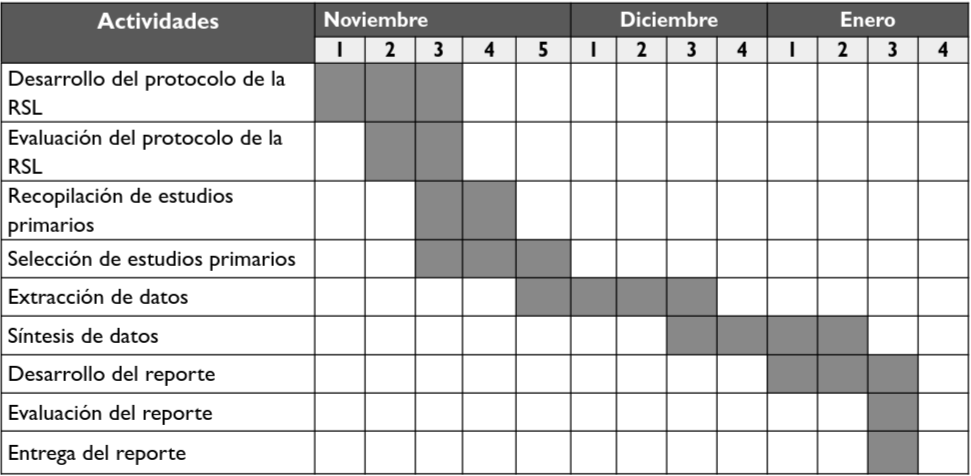
\includegraphics[width=\linewidth]{gant.png}
    \caption{Cronograma de actividades.}
    \label{fig:grant}
\end{figure}

\subsection{Herramientas utilizadas}
Se utilizó LaTex para llevar a cabo el documento del protocolo, para almacenar referencias 
se crearon diferentes archivos, los cuales contienen referencias, todos han sido 
almacenados con extensión .bib, se empleó BibTex para llevar a cabo las referencias a las 
investigaciones o documentos de interés, guardó la hoja de cálculo en la que se llevó 
a cabo búsquedas prueba y se se gestionó el proceso de control del documento con .git,
los archivos de referencias han sido alojados en GitHub,
\newpage

\subsubsection{Paquete de replicación}
Como un aporte a la comunidad de investigación en el área de ingeniería de \emph{software}, 
se añade un paquete de replicación de la investigación, con el objetivo de aportar  
al conjunto de estudiantes e investigadores interesados y de esta forma avanzar y distribuir 
conocimiento.
El paquete de replicación también será una herramienta importante utilizada con el fin de replicar 
el proceso de investigación llevado a cabo, 

Lista de items incluídos en el paquete: 
  \begin{enumerate}[(a)]
  \item Anteproyecto con descripción de objetivo y contexto de la investigación. 
  \item Lista de referencias utilizadas como fundamento de conocimiento. (.bib)
  \item Lista de referencias utilizadas en el protocolo.  (.bib)
  \item Protocolo.
  \item Tabla de \emph{Google sheets} con detalle de búsquedas piloto realizadas. 
  \item Lista de referencias utilizadas en el protocolo de investigación.
  \end{enumerate}
\newpage

\section{Referencias}

\end{document}
